\documentclass[tcn = 37075, sheet = true, abstract = true]{mcmthesis}
\problem{A}
\usepackage{palatino}
\usepackage{mwe}
\usepackage{slashbox}
\usepackage{mathrsfs}

\title{The \LaTeX Template for MCM Version 5.1.0b}
\author{\small \href{http://www.latexstudio.net/}
  {
\includegraphics[width=7cm]{mcmthesis-logo}}}
\date{\today}

\begin{document}
\begin{abstract}
\lipsum[1]
\begin{keywords}
keyword1; keyword2
\end{keywords}
\end{abstract}
\maketitle
\newpage
\section{Introduction}

\section{Setting up the Background}

(\textit{This paragraph needs rephrasing later}) Building the organizing network of the company requires first to plausibly incorporating the organizational graph (as presented in figure 1) and the allocation of different levels of positions (as indicated in table 1). To reach this, we assign different positions to different offices according to several rules. After some minor adjustments, we can get a possible and reasonable allocation of staff, on which we will build our later analysis. The assumptions related to the allocation are as follows:

\noindent \textbf{Assumptions}:

To explain the assumptions clearly, we first define terms "tree" and "tier". Tree is defined to be the whole picture of the organizational graph. Entries are defined to be in the same tier if they are on the same horizontal line in figure 1. Thus we can see that the tree stems from the higher tier of CEO to the lowest tier of branches. Now the assumptions:

\begin{itemize}
\item Every senior/junior manager should have a clerk in his/her office for administrative tasks.
\item The level of position of a staff tend to be higher when his office is closer to the CEO in the organizational graph.
\item The level of position of a staff tend to be higher when his office is the root of divisions of more people.
\item The level of position of a manager cannot be lower than someone whose office belongs to a lower tier.
\item Research tasks should be conducted by experienced employees.
\end{itemize}

Thus we can get the following table of allocation of 370 positions:
\begin{table}[htb!]
\centering
\begin{tabular}{l|lllllllll}   \hline
\backslashbox{Tier}{}& \backslashbox{Position}{level}&1&2&3&4&5&6&7&Total\\ \hline
1                  & CEO              & 2              & 0              & 0                      & 0                        & 0                    & 0                      & 2                    & 4     \\
\multirow{7}{2pt}{2} & Research           & 1              & 0              & 0                      & 0                        & 2                    & 0                      & 1                    & 4     \\
                   & CIO                & 1              & 2              & 0                      & 0                        & 8                    & 0                      & 3                    & 14    \\
                   & CFO                & 1              & 2              & 0                      & 0                        & 8                    & 0                      & 3                    & 14    \\
                   & HR                 & 0              & 1              & 0                      & 0                        & 2                    & 0                      & 1                    & 4     \\
                   & VP                 & 2              & 0              & 0                      & 0                        & 0                    & 0                      & 2                    & 4     \\
                   & Facilities         & 1              & 0              & 0                      & 0                        & 2                    & 0                      & 1                    & 4     \\
                   & Sales Marketing    & 1              & 0              & 0                      & 0                        & 2                    & 0                      & 1                    & 4     \\
 \multirow{9}{2pt}{3} & Networks           & 0              & 1              & 1                      & 0                        & 11                   & 0                      & 1                    & 14    \\
                   & Information        & 0              & 1              & 1                      & 0                        & 11                   & 0                      & 1                    & 14    \\
                   & Program Manager    & 0              & 1              & 1                      & 0                        & 6                    & 5                      & 1                    & 14    \\
                   & Production Manager & 1              & 1              & 0                      & 0                        & 10                   & 0                      & 2                    & 14    \\
                   & Plant Blue         & 0              & 1              & 1                      & 0                        & 6                    & 5                      & 1                    & 14    \\
                   & Plant Green        & 0              & 1              & 1                      & 0                        & 6                    & 5                      & 1                    & 14    \\
                   & Regional           & 0              & 1              & 1                      & 0                        & 6                    & 5                      & 1                    & 14    \\
                   & World Wide         & 0              & 1              & 1                      & 0                        & 6                    & 5                      & 1                    & 14    \\
                   & Internet           & 0              & 1              & 1                      & 0                        & 6                    & 5                      & 1                    & 14    \\
4                  & Director           & 0              & 6              & 6                      & 0                        & 6                    & 0                      & 6                    & 24    \\
5                  & Branch             & 0              & 0              & 11                     & 25                       & 12                   & 120                    & 0                    & 168   \\ \hline

&Total              & 10             & 20             & 25                     & 25                       & 110                  & 150                    & 30                   & 370 \\  \hline
\end{tabular} 

*1:Senior Manager 2:Junior Manager 3:Experienced Supervisor 4:Inexperienced Supervisor 5:Experienced Employee 6:Inexperienced Employee 7:Administrative Clerk

\caption{The distribution of staff in different positions}
\end{table}



We set up to build the network in this company. Define $V(G)=\{v_1,v_2,...v_{370}\}$ as the set of all positions. Each node denotes one position. Define $E(G)$ is the set of edges in the network. $(v_i,v_j)\in E(G)$ if at least one of the following holds:


\begin{itemize}
\item $i$ and $j$ are in the same office. Here one entry in figure 1 is considered as an office, whether it consists of two divisions of 14 staff members or only four staff members.
\item $i$ is the head of an office and $j$ is the head of the directly-related upper office or the opoosite. Here the staff in the highest level of position within an office is considered as the head of the office, such as the junior manager in Networks office and the experienced supervisor in Branch office.
\item $i$ and $j$ are both senior manager or junior manager.
\end{itemize}

$G=\{V(G),E(G)\}$ is the the graph of this network. We then visualize the network in the following picture (figure 1).

\textbf{input the Gephi graph}

\begin{figure}[htb!]
\small
\centering
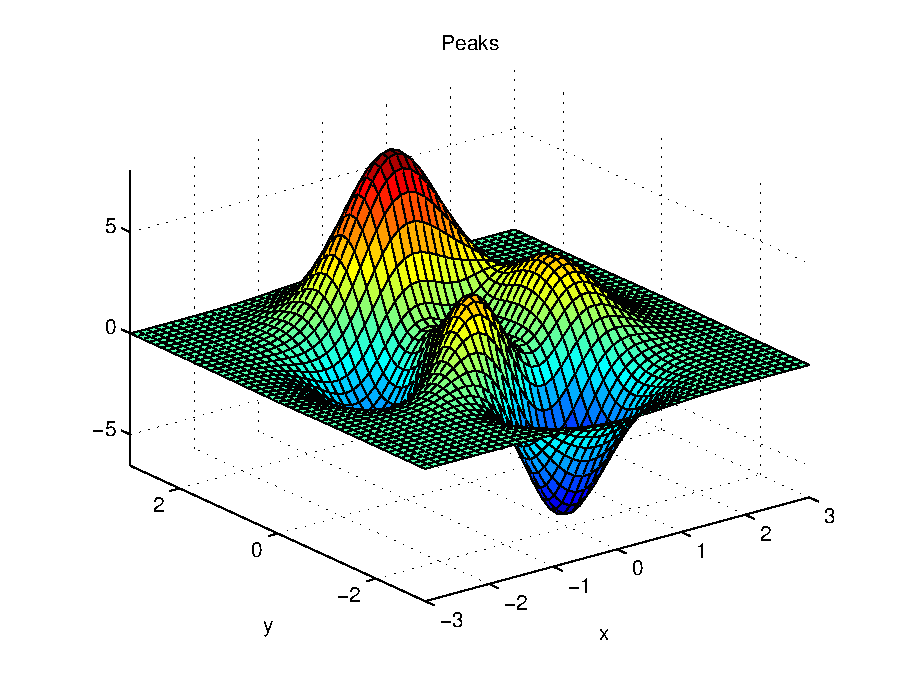
\includegraphics[width=12cm]{mcmthesis-aaa.eps}
\caption{aa} \label{fig:aa}
\end{figure}

Then we turn to the main part of building up our model and using it for analysis. To deal with the complicated real problems, we first simplify them into two process. The first process is named as "output" and the second process is named "input". Like in the real world and in the problem, the "output" process refers to the situations where the staff leave his or her position. The "input" process, accordingly, refers to the combination of internal promotion and outsourcing recruitment. The formal models are presented in the next section. Based on this process division, we can easily see that the "input" process is where the Human Resource manager works his or her power to control and improve the company's current position.


\section{Models}

We hold the intention to create a dynamic model which can be controlled by manipulating some of the parameters. Specially, we assume that the "output" process is largely determined by individual characteristics rather than company's policy. However, we also want to create a set of tools that human resource managers can use to deal with the possible staff problems. With these in mind, we design two models that capture the process of "output" with different emphasis and simulate three possible strategy for the human resource manager: purely recruiting, purely promoting and the "greedy" strategy. These models and simulations will help to solve the task 1-5 and even dig deeper insights about staff management. 

To begin with, define $\Omega^{(t)}$ as the set of people who leave the company in period $t$, $\Theta^{(t)}$ as the set of people who is recruited in period $t$ and $\Gamma^{(t)}$ as the set of people who work in the company at the beginning of period $t$. $\Gamma^{(t)}$ can be seen as a subset of $V(G)$, but the former indicates people and the later indicates positions. It's obvious that $\Gamma^{(t)}=\Gamma^{(t-1)}\bigcup \Theta ^{(t-1)} \backslash \Omega^{(t-1)}$. Next we consider two ways of capturing churn.

\subsection{Understanding "Output"}
\subsubsection{}{Model I : Capture Churn Using Information Accumulation}

\paragraph{Information Effect}
In this model, we capture the way an individual is influenced by other people's leaving using information flow. In other words, the event of one person leaves acts as a influential message, transmitting across the network built earlier. We call it information effect. We assume that the information effect will accumulate, that is, the churn news this month and last month will have an equal and add-up influence in shaping the listen's decision. In order to make the model easier to control, we add an assumption that the a piece of information's effect will expire after six months. This modeling technique can be justified by the psychological evidence (\textbf{where to find any???}) that . To formalize this process in mathematical expressions, we first define some metric to measure the information effect. 

\begin{itemize}
\item Influence: The resign of staff in different level of positions has different influence. For example, the churn of a senior manager tend to have greater impact on one's decision compared with the churn of an inexperienced employee. We denote the influence by $e_i$, $i=1,2,...,7$.
\item Distance: The distance between two nodes $i$ and $j$ is defined by the shortest path connecting $i$ and $j$ in the graph. It is the shortest possible way that the churn of $i$ reaches $j$. We denote it by $d_{ij}$.
\item Information effect is proportional to the influence.
\item Information effect is inversely proportional to the squared distance.
\item Information effect is accumulated for the past six months.
\end{itemize}

Formally, the information effect on individual $i\in \Gamma{(t)}$ can be calculated as follows:
$$\displaystyle \sum_{\tau=t-6}^{t-1}\sum_{j\in \Omega^{(\tau)}}\frac{e_j^{(\tau)}}{d_{ij}^{(\tau)2}}$$

\paragraph{Tenure Effect}
Another aspect we take into consideration is called tenure effect. \textbf{where to find any???} The longer an individual stays in the same position, the more likely he/she is to be dissatisfied with his current condition. We add a multiplier before the information effect to incorporate this additional effect. Besides, tenure effect tend to increase faster as tenure increases. So we simply adopt the quadratic form.

Combine information effect and tenure effect, we develop a measure called "dissatisfaction" $\sigma_i^{(t)}$:

$$\displaystyle \sigma_i^{(t)}=(1+kt_i^{(t)2})*\sum_{\tau=t-6}^{t-1}\sum_{j\in \Omega^{(\tau)}}\frac{e_j^{(\tau)}}{d_{ij}^{(\tau)2}}~~~~\forall i\in \Gamma{(t)}
$$

Here $t_i^{(t)}$ is the length of individual $i$ has stayed in his current position at time $t$ and $k$ is the control parameter. 

\paragraph{Tolerance Threshold}
For each individual, he has an internal tolerant threshold $\zeta_i$. When his dissatisfaction measure exceeds his threshold and he is not promoted, he will decide to leave this company. Tolerant threshold is not necessarily a fixed value. We assume it is uniformly distributed in the interval $[m_i-\frac{1}{2\alpha m_i},m_i+\frac{1}{2\alpha m_i}]$. We further assume common middle point $m_i$ for all individuals in the same level of position.



\subsubsection{Model II : Capture Churn Using Bayesian Learning}

Another way of capturing the effect from others can is to interpreted it as a learning process, which is widely discussed in network science and economics literature (\textbf{to be precise???}Jackson 2013; Acemoglu 2008;). The main context for this kind of modeling lies in that individuals perceives two states of the world or actions and act in response based on Bayesian inference. In the settings of this problem, this two states are \textit{to leave} or \textit{to stay}.


\subsection{Understanding "Input"}

In this part, we combine two parts that a HR manager can control, namely supplement strategies and experience requirements, define the "input" in our model. To be more specific,  strategies here are the schemes of both promotions and recruitment. They are combinedly referred to as "recruitment strategy". The two most easily named strategies are purely promoting strategy and purely recruiting strategy

\subsection{Simulations}



\subsection{Model Extensions}

There are several possible extensions to the models we have described before. These extensions are used to modify some of the bold but kind of restrictive assumptions made before and help to come closer to reality. Note that some of these new extensions need information about the real data of the company. Besides, being more precise means in the other direction that the extended models will not be as powerful and encompassing as the baseline models. Though the insights they are shedding lights on are basically the same.

\subsubsection{}


\begin{equation}
a^2 \label{aa}
\end{equation}

\[
  \begin{pmatrix}{*{20}c}
  {a_{11} } & {a_{12} } & {a_{13} }  \\
  {a_{21} } & {a_{22} } & {a_{23} }  \\
  {a_{31} } & {a_{32} } & {a_{33} }  \\
  \end{pmatrix}
  = \frac{{Opposite}}{{Hypotenuse}}\cos ^{ - 1} \theta \arcsin \theta
\]
\lipsum[9]

\[
  p_{j}=\begin{cases} 0,&\text{if $j$ is odd}\\
  r!\,(-1)^{j/2},&\text{if $j$ is even}
  \end{cases}
\]

\lipsum[10]

\[
  \arcsin \theta  =
  \mathop{{\int\!\!\!\!\!\int\!\!\!\!\!\int}\mkern-31.2mu
  \bigodot}\limits_\varphi
  {\mathop {\lim }\limits_{x \to \infty } \frac{{n!}}{{r!\left( {n - r}
  \right)!}}} \eqno (1)
\]





We measure a worker's productivity according to his dissatisfaction:
$$p_i^{(t)}=e^{-d_i^{(t)}}$$

The productivity of the firm is the sum of productivity of total individuals:
$$P^{(t)}=\sum i\in \Gamma{(t)} $$


\section{MLE Estimation of the Parameters}

In this part, we briefly discuss how to estimate the parameter in Model 1 if we have additional information.

The unknown parameters are: the influence of different levels of position $e_i$ in the network $e_i$, the parameters depicting the distribution of tolerant threshold in different levels of position $m_i$ and $\alpha$ and the control parameter $k$ in tenure effect.

At time $t$, individual $i$ has dissatisfaction measure:

$$\displaystyle \sigma_i^{(t)}=(1+kt_i^{(t)2})*\sum_{\tau=t-6}^{t-1}\sum_{j\in \Omega^{(\tau)}}\frac{e_j^{(\tau)}}{d_{ij}^{(\tau)2}}~~~~\forall i\in \Gamma{(t)}
$$

The probability that individual $i$ will resign in time $t$ can be calculated as follows:

$$\displaystyle p_i^{(t)}=P(\sigma_i^{(t)}>\zeta_i)=1-P(\sigma_i^{(t)}<\zeta_i)=\frac{1}{2}+\alpha m_i(m_i-\sigma_i^{(t)})$$

We should maximize the following expression:

$$\prod\limits_{i \in \Omega^{(t)}} p_i \prod_{i\in \Gamma^{(t)}\backslash \Omega^{(t)}}(1-p_i)$$

that is:

$$\max \limits_{\{e_i\}_{i=1}^7,\{m_i\}_{i=1}^7,k} \prod_{i \in \Omega^{(t)}} (\frac{1}{2}+\alpha m_i(m_i-(1+kt_i^{(t)2})*\sum_{\tau=t-6}^{t-1}\sum_{j\in \Omega^{(\tau)}}\frac{e_j^{(\tau)}}{d_{ij}^{(\tau)2}}) ) $$ 
$$~~~~~~~~~~~~~~~~~~~~~~~~*\prod_{i\in \Gamma^{(t)}\backslash \Omega^{(t)}}(\frac{1}{2}-\alpha m_i(m_i-(1+kt_i^{(t)2})*\sum_{\tau=t-6}^{t-1}\sum_{j\in \Omega^{(\tau)}}\frac{e_j^{(\tau)}}{d_{ij}^{(\tau)2}}) ) $$

If we have collected data for the past $N$ months about the "input" and "output" of this company, we can multiply them together and take natural logarithm. Then it is equivalent to solve the following problem:

$$\max \limits_{\{e_i\}_{i=1}^7,\{m_i\}_{i=1}^7,k} \sum\limits_{\tau=t-N}^{t-1} \sum_{i \in \Omega^{(t)}} \ln (\frac{1}{2}+\alpha m_i(m_i-(1+kt_i^{(t)2})*\sum_{\tau=t-6}^{t-1}\sum_{j\in \Omega^{(\tau)}}\frac{e_j^{(\tau)}}{d_{ij}^{(\tau)2}}) ) $$ 
$$~~~~~~~~~~~~~~~~~~~~~~~~+\sum\limits_{\tau=t-N}^{t-1} \sum\limits_{i \in \Gamma^{(t)} \backslash \Omega^{(t)}} \ln (\frac{1}{2}-\alpha m_i(m_i-(1+kt_i^{(t)2})*\sum_{\tau=t-6}^{t-1}\sum_{j\in \Omega^{(\tau)}}\frac{e_j^{(\tau)}}{d_{ij}^{(\tau)2}}) ) $$

We can then adopt the 


\section{The Model Results}
\lipsum[6]

\section{}
\lipsum[9]

\section{Conclusions}
\lipsum[6]

\section{A Summary}
\lipsum[6]

\section{Evaluate of the Mode}

\section{Strengths and weaknesses}
\lipsum[12]

\subsection{Strengths}
\begin{itemize}
\item \textbf{Applies widely}\\
This  system can be used for many types of airplanes, and it also
solves the interference during  the procedure of the boarding
airplane,as described above we can get to the  optimization
boarding time.We also know that all the service is automate.
\item \textbf{Improve the quality of the airport service}\\
Balancing the cost of the cost and the benefit, it will bring in
more convenient  for airport and passengers.It also saves many
human resources for the airline. \item \textbf{}
\end{itemize}

\begin{thebibliography}{99}
\bibitem{1} D.~E. KNUTH   The \TeX{}book  the American
Mathematical Society and Addison-Wesley
Publishing Company , 1984-1986.
\bibitem{2}Lamport, Leslie,  \LaTeX{}: `` A Document Preparation System '',
Addison-Wesley Publishing Company, 1986.
\bibitem{3}\url{http://www.latexstudio.net/}
\bibitem{4}\url{http://www.chinatex.org/}
\end{thebibliography}

\begin{appendices}

\section{First appendix}

\lipsum[13]

Here are simulation programmes we used in our model as follow.\\

\textbf{\textcolor[rgb]{0.98,0.00,0.00}{Input matlab source:}}
\lstinputlisting[language=Matlab]{./code/mcmthesis-matlab1.m}

\section{Second appendix}

some more text \textcolor[rgb]{0.98,0.00,0.00}{\textbf{Input C++ source:}}
\lstinputlisting[language=C++]{./code/mcmthesis-sudoku.cpp}

\end{appendices}

\end{document}

